% 6.3 Results
\subsection{Results}
Two separate methods were used to calculate the size distribution of
segmented particles resulting from different segmentations on the
same F50 sand and Kel-F CT scan.
Segmented particles were analyzed for watershed segmentations seeded with
markers determined with minimum peak distance values ranging from 4 to 8.
These values correlate to physical distances from 55.36 to 110.72 µm.
Each method determined whether or not a particle would be retained in a
separate way.
The first method
used spheres of equivalent volume for each segmented particle. The second
method used the aspect ratio of the bounding box of each particle.
To determine which minimum peak distance resulted in the most accurate size
distribution, each segmentation is compared with the
standard size distribution of F50 sand (\ref{fig/06/f50}).

\begin{figure}[ht]
    \centering
    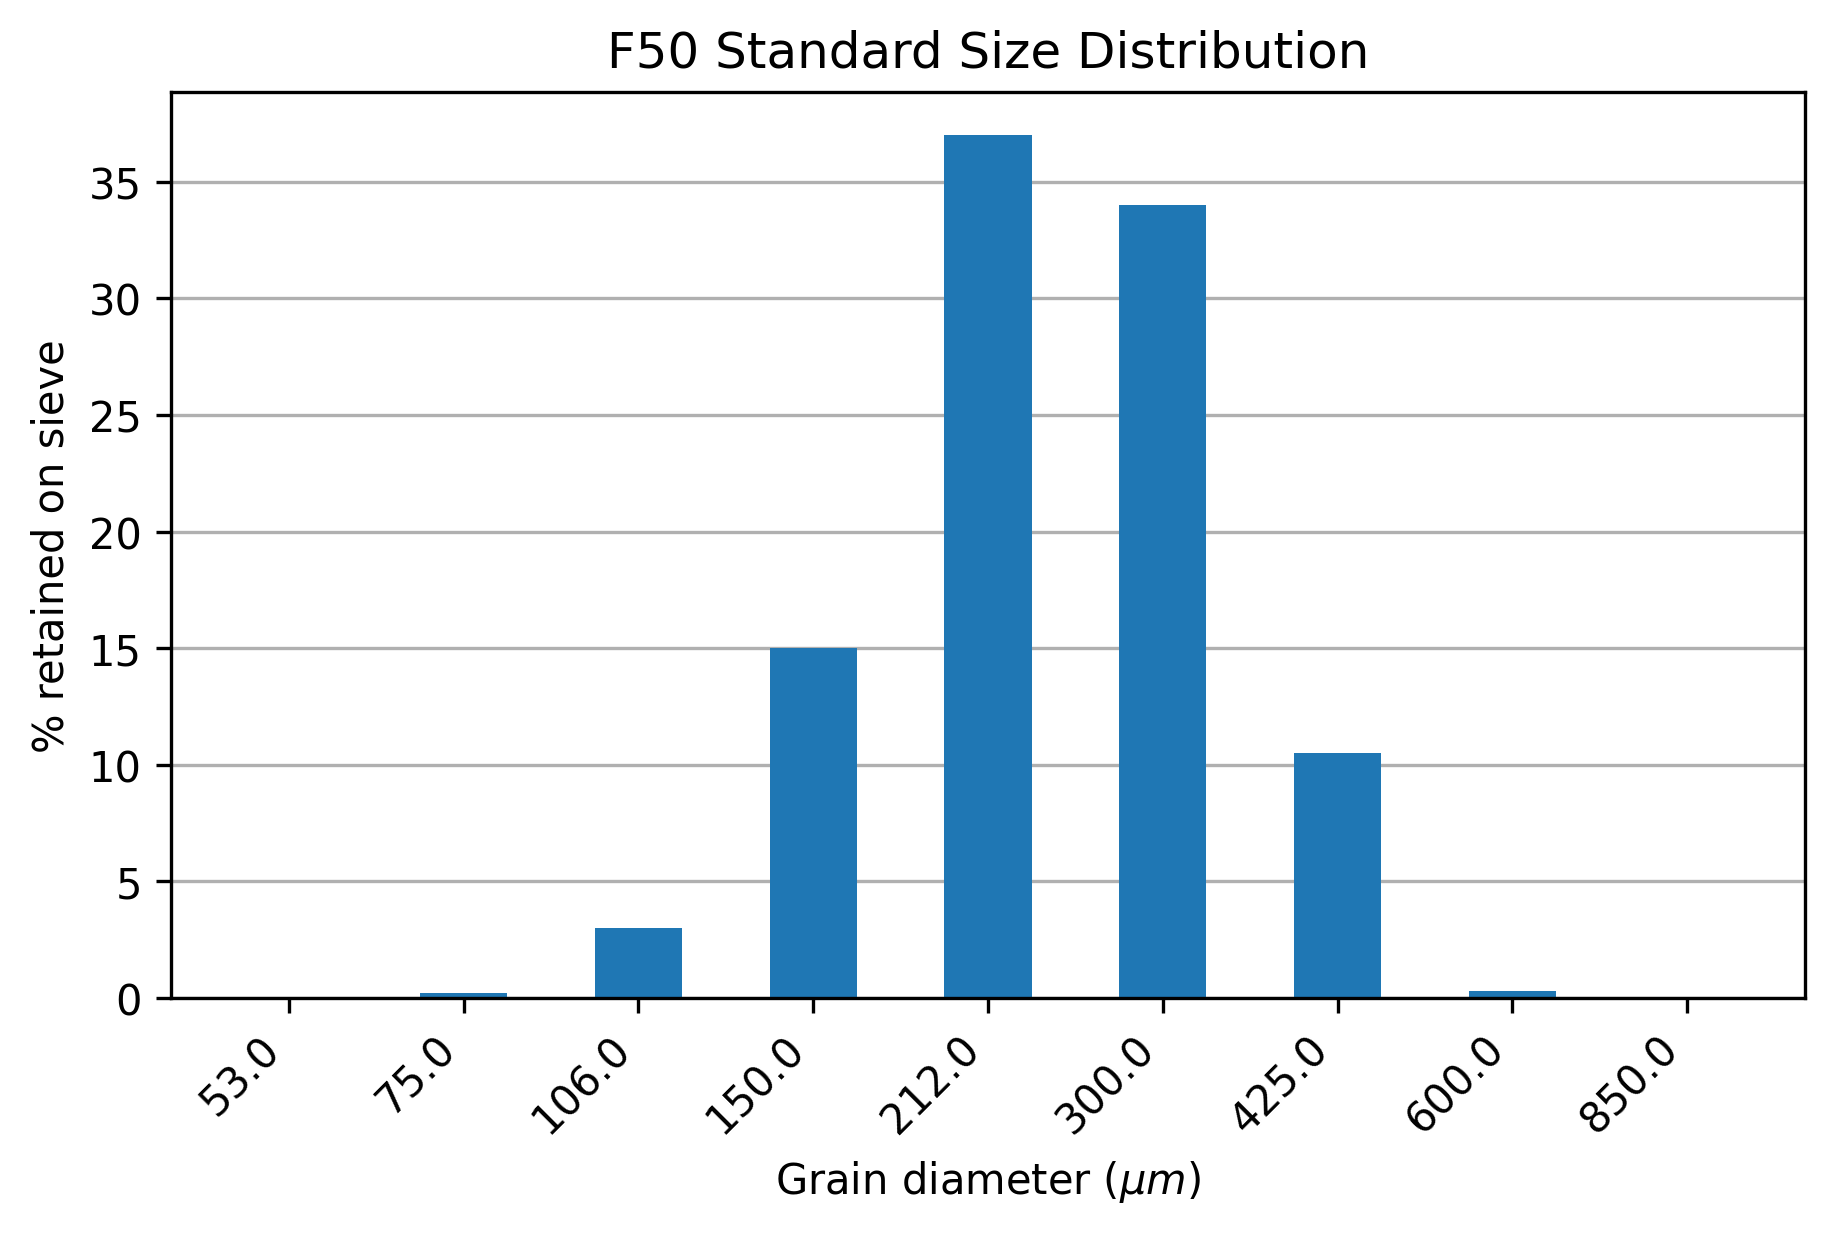
\includegraphics[width=0.75\textwidth]{figures/06/03-f50-size.png}
    \caption{
        \small\setstretch{1}
        Expected result from passing F50 sand through a series of sieves,
        expressed in percent of total grains retained at each step. Sieve
        size is given in microns.
    }
    \label{fig/06/f50}
\end{figure}

\subsubsection{Sphere of Equivalent Volume to Determine Size}
% -------------------------------------------------------------------------
The first method method for calculating segmented particle size distribution
took the volume of each particle,
calculated the diameter of the sphere with an equivalent volume, and used this
diameter to bin the particles between sieve mesh sizes
(\ref{fig/06/sphere}). The error between each
of the five segmentations was calculated as the cumulative difference between
the equivalent sphere distribution and the typical F50 distribution. These
errors are summarized for each segmentation in Table \ref{tab/06/error}.
The segmented particles seeded with a 6 pixel minimum peak distance has the
lowest error with a cumulative difference of 25.08\%. Particles seeded with
a 4 pixel minimum peak distance had the largest error at 79.29\%.

\begin{figure}[ht]
    \centering
    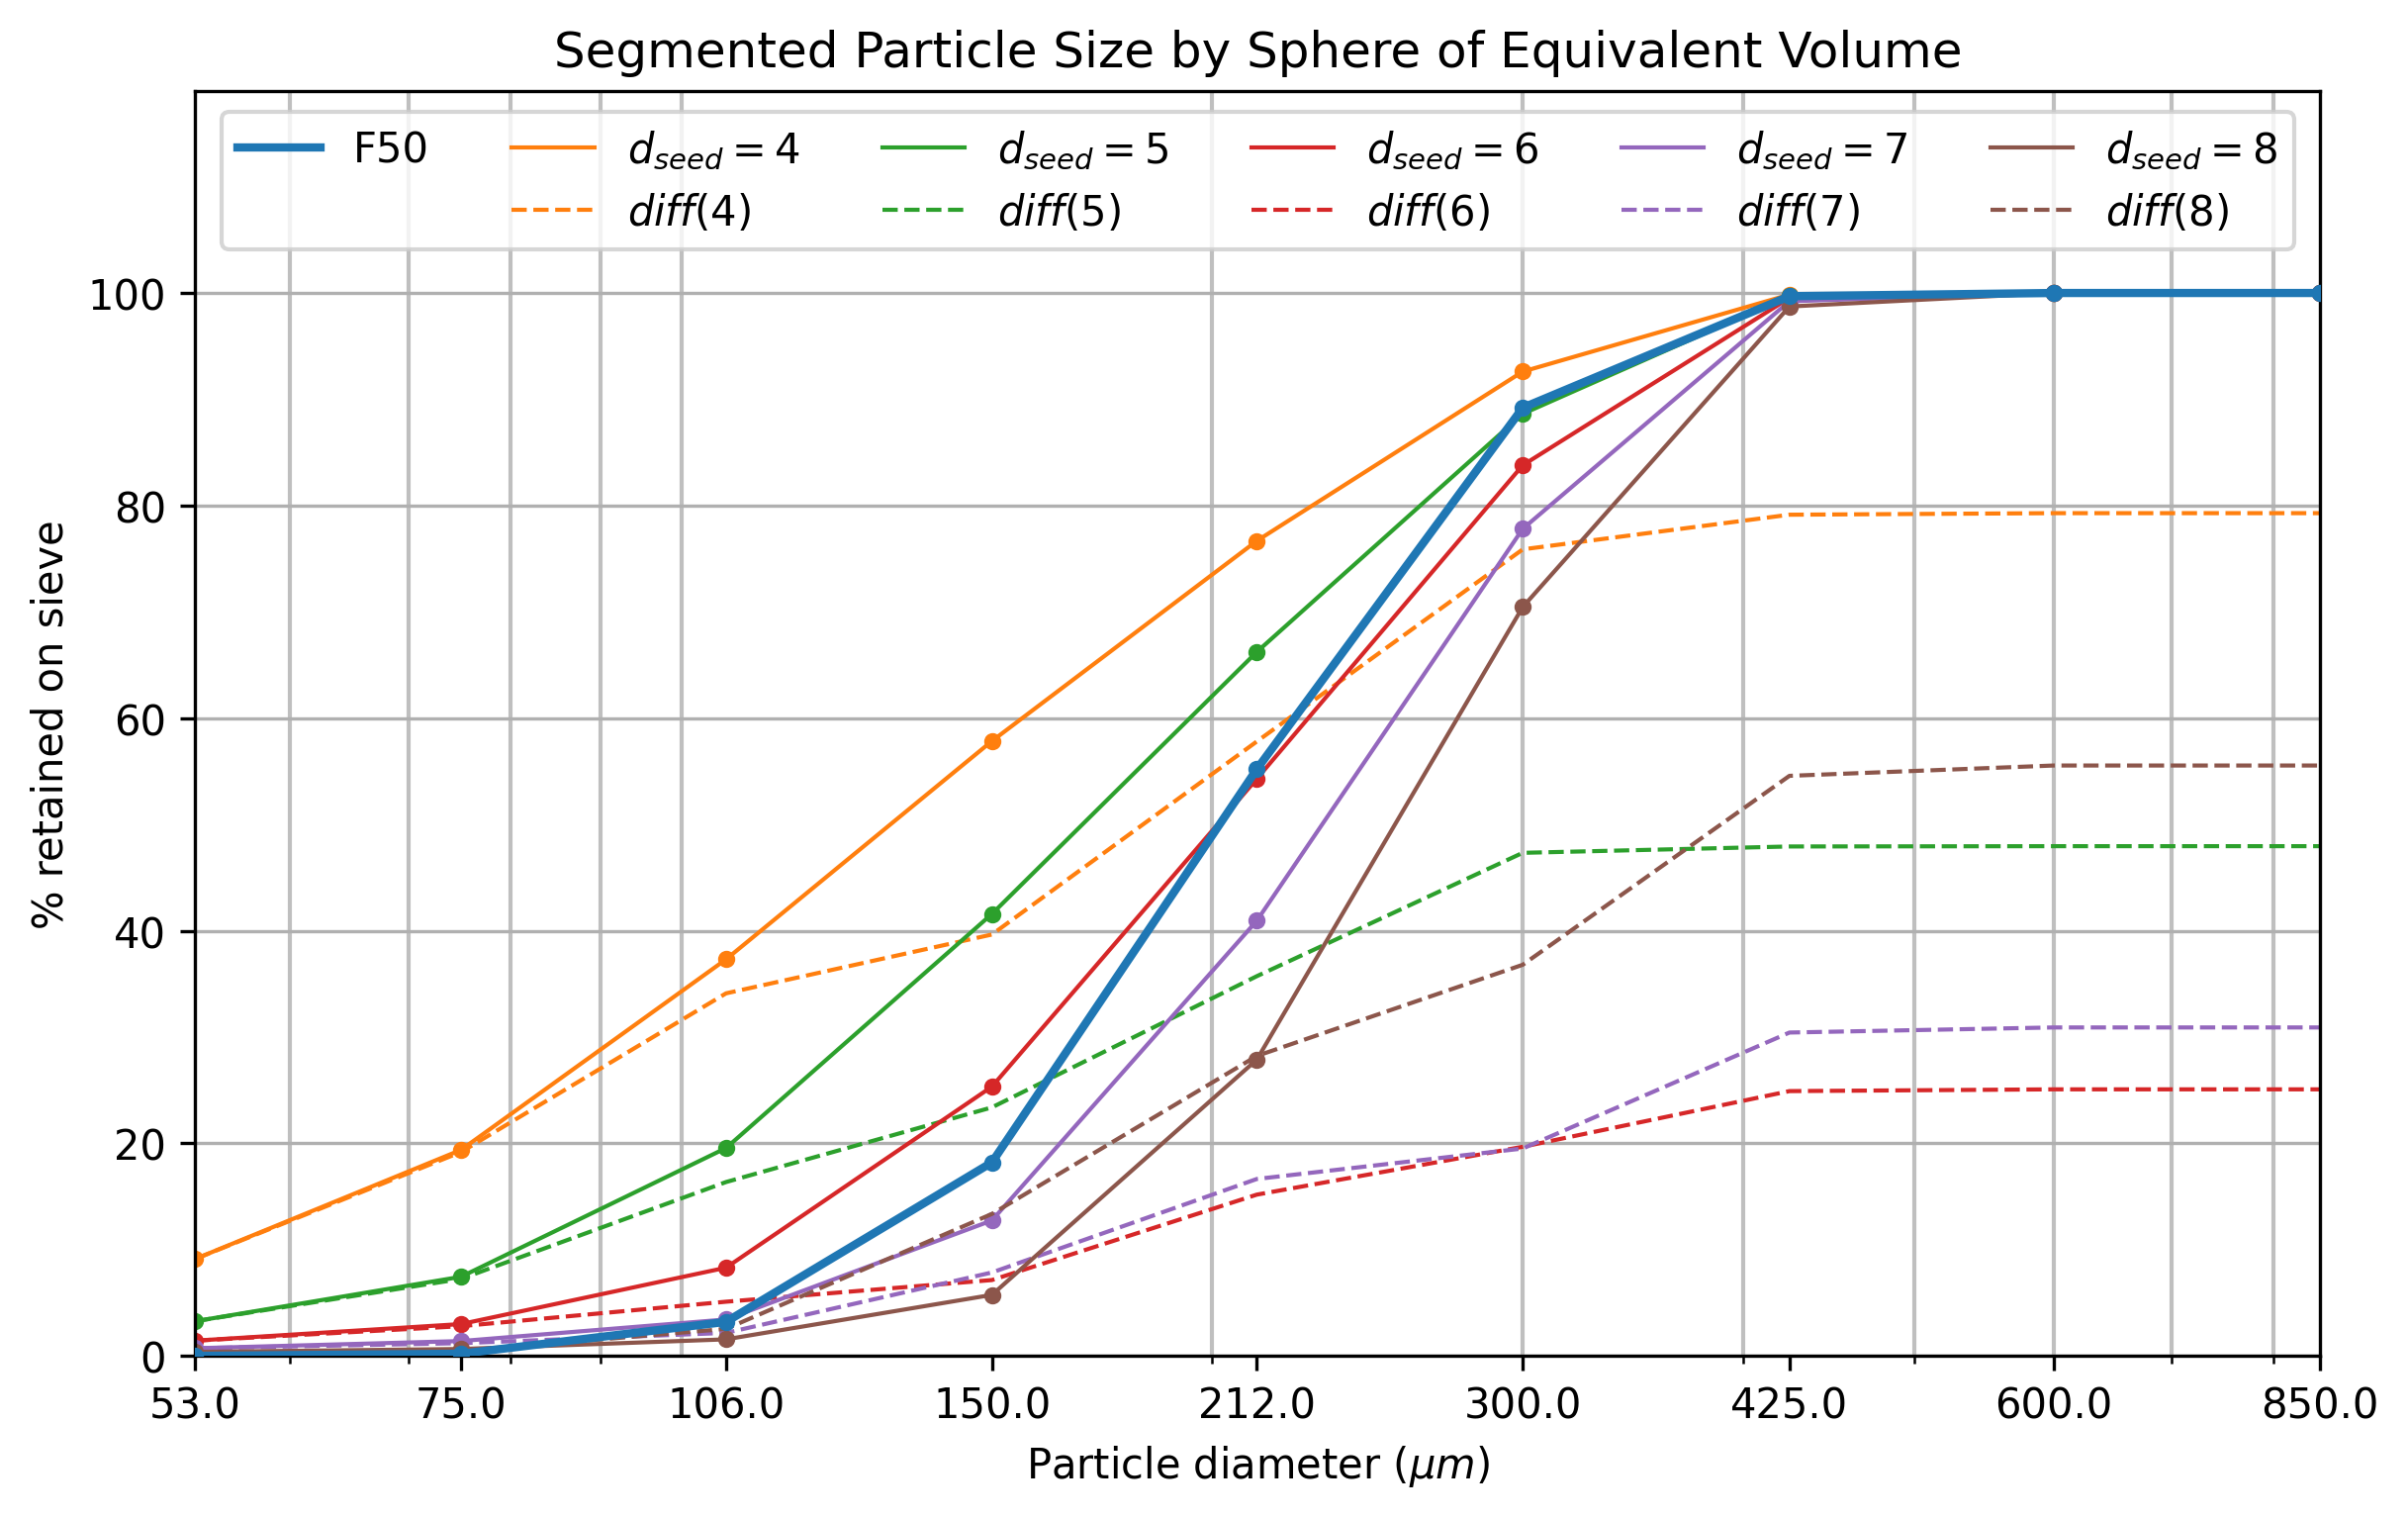
\includegraphics[width=0.75\textwidth]{figures/06/04-size-by-sphere.png}
    \caption{
        \small\setstretch{1}
        Size distribution of segmented particles binned
        according to the sphere of equivalent volume of each particle.
        Solid lines represent the cumulative distribution of particles at
        increasing sieve sizes. The blue solid line represents the typical
        values for F50 sand and the other solid lines represent the values
        determined from the particles obtained by segmenting the CT scan
        with a watershed algorithm seeded with different values for the
        minimum peak distance ($d_{seed}$). Dashed lines of corresponding
        color represent the error between the segmentation and typical values.
    }
    \label{fig/06/sphere}
\end{figure}

\subsubsection{Aspect Ratio of Bounding Box to Determine Size}
% -------------------------------------------------------------------------
The second method for calculating segmented particle size distribution
found the aspect ratio of the bounding box of each segmented particle and
used the maximum length of the minimum cross sectional area to bin the
particles (\ref{fig/06/aspect}). Just like with the equivalent sphere
method, the error between each
of the five segmentations was calculated as the cumulative difference between
the equivalent sphere distribution and the typical F50 distribution.
These errors are also summarized for each segmentation in Table \ref{tab/06/error}.
With this method of assessing the segmentations, the
particles segmented with a 5 pixel minimum peak distance have the lowest
error with a cumulative difference of 45.31\%. Particles seeded with an
8 pixel minimum peak distance had the largest error at nearly 95.59\%.

\begin{figure}[ht]
    \centering
    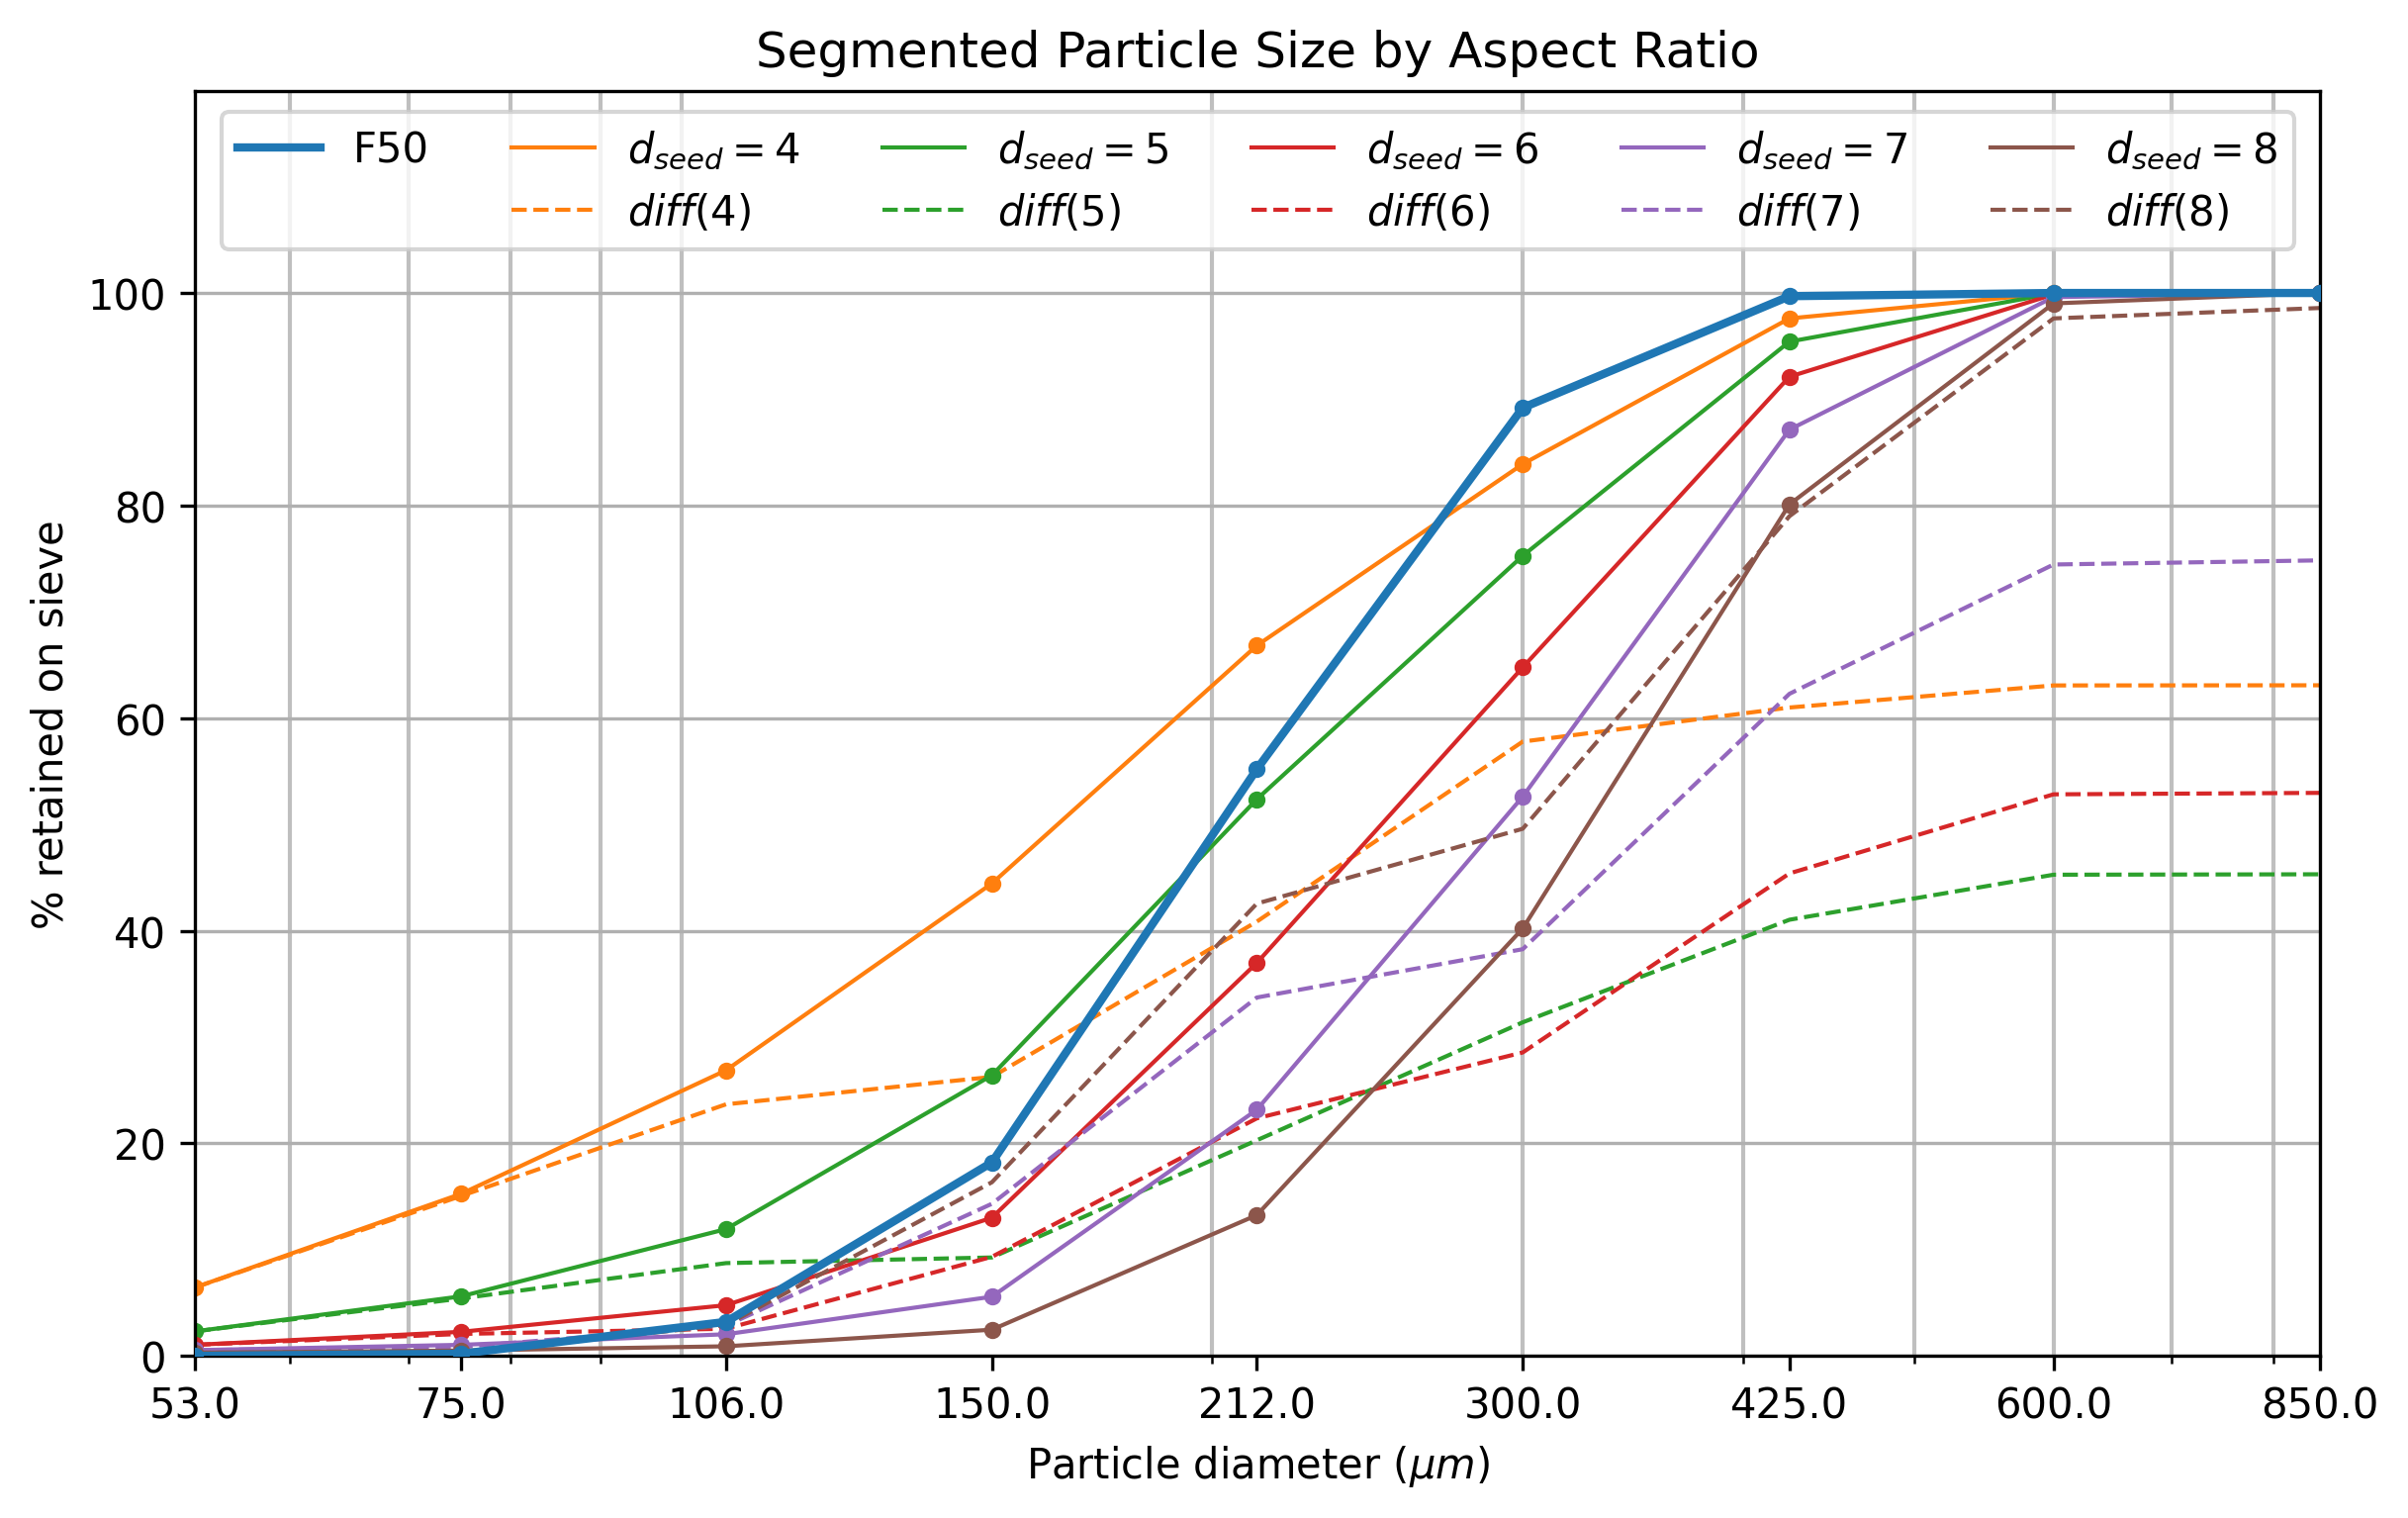
\includegraphics[width=0.75\textwidth]{figures/06/05-size-by-aspect.png}
    \caption{
        \small\setstretch{1}
        Size distribution of segmented particles binned
        according to the bounding box aspect ratio of each particle.
        Solid lines represent the cumulative distribution of particles at
        increasing sieve sizes. The blue solid line represents the typical
        values for F50 sand and the other solid lines represent the values
        determined from the particles obtained by segmenting the CT scan
        with a watershed algorithm seeded with different values for the
        minimum peak distance ($d_{seed}$). Dashed lines of corresponding
        color represent the error between the segmentation and typical values.
    }
    \label{fig/06/aspect}
\end{figure}

The sum of absolute errors for each segmentation are summarized in Table
\ref{tab/06/error}, combining
each method of determining the particle size, as well as the total error
which is the sum of the error from both methods. Based on these errors, the
watershed segmentation seeded with markers determined by a 6 pixel minimum peak
distance yields the results that most closely align with the typical F50 sand
size distribution.

\begin{table}[ht]
    \centering
    \caption{Segmented Particle Errors Relative to Typical F50 Sand}
    \label{tab/06/error}
    \renewcommand{\arraystretch}{1.5}% Spread rows out...
    \begin{tabular}{|>{\centering\bfseries}m{1in} >{\centering}m{0.75in} >{\centering}m{0.75in} >{\centering}m{0.75in} >{\centering}m{0.75in} >{\centering\arraybackslash}m{0.75in}|}
        \hline % \toprule
        Error             & \textbf{d\textsubscript{seed} = 4} & \textbf{d\textsubscript{seed} = 5} & \textbf{d\textsubscript{seed} = 6} & \textbf{d\textsubscript{seed} = 7} & \textbf{d\textsubscript{seed} = 8} \\
        \hline % \midrule
        Equivalent Sphere &  79.29 & 47.95 & 25.08 &  30.90 &  55.54 \\
        Aspect Ratio      &  63.09 & 45.31 & 52.97 &  74.84 &  95.59 \\
        Total             & 142.38 & 93.26 & 78.05 & 105.74 & 154.13 \\
        \hline % \bottomrule
    \end{tabular}
\end{table}

Using the optimal parameter as determined by measuring the size distributions,
this segmentation is used to generate surface meshes for the entire sample.

\begin{figure}[ht]
    \centering
    \includegraphics[width=0.9\textwidth]{figures/06/07-full-41553_particles.png}
    \caption{
        \small\setstretch{1}
        Surface meshes of all 41,553 particles segmented from the F50 sand
        sample loaded from three different views:
        (a) the top, (b) a high angle, and (c) the side.
    }
    \label{fig/06/full}
\end{figure}

